% Options for packages loaded elsewhere
\PassOptionsToPackage{unicode}{hyperref}
\PassOptionsToPackage{hyphens}{url}
%
\documentclass[
]{article}
\usepackage{amsmath,amssymb}
\usepackage{lmodern}
\usepackage{iftex}
\ifPDFTeX
  \usepackage[T1]{fontenc}
  \usepackage[utf8]{inputenc}
  \usepackage{textcomp} % provide euro and other symbols
\else % if luatex or xetex
       %%% MODIFIED: unicode-math conflics with expex; mathspects conflicts with glossaries/leipzig
  \usepackage{fontspec} % \usepackage{unicode-math}
  \defaultfontfeatures{Scale=MatchLowercase}
  \defaultfontfeatures[\rmfamily]{Ligatures=TeX,Scale=1}
  \setmainfont[]{DejaVu Sans}
\fi
% Use upquote if available, for straight quotes in verbatim environments
\IfFileExists{upquote.sty}{\usepackage{upquote}}{}
\IfFileExists{microtype.sty}{% use microtype if available
  \usepackage[]{microtype}
  \UseMicrotypeSet[protrusion]{basicmath} % disable protrusion for tt fonts
}{}
\makeatletter
\@ifundefined{KOMAClassName}{% if non-KOMA class
  \IfFileExists{parskip.sty}{%
    \usepackage{parskip}
  }{% else
    \setlength{\parindent}{0pt}
    \setlength{\parskip}{6pt plus 2pt minus 1pt}}
}{% if KOMA class
  \KOMAoptions{parskip=half}}
\makeatother
\usepackage{xcolor}
\IfFileExists{xurl.sty}{\usepackage{xurl}}{} % add URL line breaks if available
\IfFileExists{bookmark.sty}{\usepackage{bookmark}}{\usepackage{hyperref}}
\hypersetup{
  pdftitle={QML - Summative Assessment 1},
  pdfauthor={YOUR EXAM NUMBER},
  hidelinks,
  pdfcreator={LaTeX via pandoc}}
\urlstyle{same} % disable monospaced font for URLs
\usepackage[margin=1in]{geometry}
\usepackage{color}
\usepackage{fancyvrb}
\newcommand{\VerbBar}{|}
\newcommand{\VERB}{\Verb[commandchars=\\\{\}]}
\DefineVerbatimEnvironment{Highlighting}{Verbatim}{commandchars=\\\{\}}
% Add ',fontsize=\small' for more characters per line
\usepackage{framed}
\definecolor{shadecolor}{RGB}{248,248,248}
\newenvironment{Shaded}{\begin{snugshade}}{\end{snugshade}}
\newcommand{\AlertTok}[1]{\textcolor[rgb]{0.94,0.16,0.16}{#1}}
\newcommand{\AnnotationTok}[1]{\textcolor[rgb]{0.56,0.35,0.01}{\textbf{\textit{#1}}}}
\newcommand{\AttributeTok}[1]{\textcolor[rgb]{0.13,0.29,0.53}{#1}}
\newcommand{\BaseNTok}[1]{\textcolor[rgb]{0.00,0.00,0.81}{#1}}
\newcommand{\BuiltInTok}[1]{#1}
\newcommand{\CharTok}[1]{\textcolor[rgb]{0.31,0.60,0.02}{#1}}
\newcommand{\CommentTok}[1]{\textcolor[rgb]{0.56,0.35,0.01}{\textit{#1}}}
\newcommand{\CommentVarTok}[1]{\textcolor[rgb]{0.56,0.35,0.01}{\textbf{\textit{#1}}}}
\newcommand{\ConstantTok}[1]{\textcolor[rgb]{0.56,0.35,0.01}{#1}}
\newcommand{\ControlFlowTok}[1]{\textcolor[rgb]{0.13,0.29,0.53}{\textbf{#1}}}
\newcommand{\DataTypeTok}[1]{\textcolor[rgb]{0.13,0.29,0.53}{#1}}
\newcommand{\DecValTok}[1]{\textcolor[rgb]{0.00,0.00,0.81}{#1}}
\newcommand{\DocumentationTok}[1]{\textcolor[rgb]{0.56,0.35,0.01}{\textbf{\textit{#1}}}}
\newcommand{\ErrorTok}[1]{\textcolor[rgb]{0.64,0.00,0.00}{\textbf{#1}}}
\newcommand{\ExtensionTok}[1]{#1}
\newcommand{\FloatTok}[1]{\textcolor[rgb]{0.00,0.00,0.81}{#1}}
\newcommand{\FunctionTok}[1]{\textcolor[rgb]{0.13,0.29,0.53}{\textbf{#1}}}
\newcommand{\ImportTok}[1]{#1}
\newcommand{\InformationTok}[1]{\textcolor[rgb]{0.56,0.35,0.01}{\textbf{\textit{#1}}}}
\newcommand{\KeywordTok}[1]{\textcolor[rgb]{0.13,0.29,0.53}{\textbf{#1}}}
\newcommand{\NormalTok}[1]{#1}
\newcommand{\OperatorTok}[1]{\textcolor[rgb]{0.81,0.36,0.00}{\textbf{#1}}}
\newcommand{\OtherTok}[1]{\textcolor[rgb]{0.56,0.35,0.01}{#1}}
\newcommand{\PreprocessorTok}[1]{\textcolor[rgb]{0.56,0.35,0.01}{\textit{#1}}}
\newcommand{\RegionMarkerTok}[1]{#1}
\newcommand{\SpecialCharTok}[1]{\textcolor[rgb]{0.81,0.36,0.00}{\textbf{#1}}}
\newcommand{\SpecialStringTok}[1]{\textcolor[rgb]{0.31,0.60,0.02}{#1}}
\newcommand{\StringTok}[1]{\textcolor[rgb]{0.31,0.60,0.02}{#1}}
\newcommand{\VariableTok}[1]{\textcolor[rgb]{0.00,0.00,0.00}{#1}}
\newcommand{\VerbatimStringTok}[1]{\textcolor[rgb]{0.31,0.60,0.02}{#1}}
\newcommand{\WarningTok}[1]{\textcolor[rgb]{0.56,0.35,0.01}{\textbf{\textit{#1}}}}
\usepackage{longtable,booktabs,array}
\usepackage{calc} % for calculating minipage widths
% Correct order of tables after \paragraph or \subparagraph
\usepackage{etoolbox}
\makeatletter
\patchcmd\longtable{\par}{\if@noskipsec\mbox{}\fi\par}{}{}
\makeatother
% Allow footnotes in longtable head/foot
\IfFileExists{footnotehyper.sty}{\usepackage{footnotehyper}}{\usepackage{footnote}}
\makesavenoteenv{longtable}
\usepackage{graphicx}
\makeatletter
\def\maxwidth{\ifdim\Gin@nat@width>\linewidth\linewidth\else\Gin@nat@width\fi}
\def\maxheight{\ifdim\Gin@nat@height>\textheight\textheight\else\Gin@nat@height\fi}
\makeatother
% Scale images if necessary, so that they will not overflow the page
% margins by default, and it is still possible to overwrite the defaults
% using explicit options in \includegraphics[width, height, ...]{}
\setkeys{Gin}{width=\maxwidth,height=\maxheight,keepaspectratio}
% Set default figure placement to htbp
\makeatletter
\def\fps@figure{htbp}
\makeatother
\setlength{\emergencystretch}{3em} % prevent overfull lines
\providecommand{\tightlist}{%
  \setlength{\itemsep}{0pt}\setlength{\parskip}{0pt}}
\setcounter{secnumdepth}{5}
\ifLuaTeX
  \usepackage{selnolig}  % disable illegal ligatures
\fi

\title{QML - Summative Assessment 1}
\author{YOUR EXAM NUMBER}
\date{2023-10-18}

\begin{document}
\maketitle

\section{Instructions}\label{instructions}

\textbf{PLEASE READ CAREFULLY}

\textbf{DUE Week 8 - Thu 9 November at noon}

You must include your \textbf{exam number as the author} in the document
preamble above.

You'll notice that line 10 of the preamble says
\texttt{mainfont:\ DejaVu\ Sans}. We would appreciate it if you'd use
this font (or at least some other sans-serif font). \textbf{Try to
render this Rmd file now, before making any changes, to see if you have
this font installed.}

\begin{itemize}
\tightlist
\item
  If you get an error message saying that DejaVu Sans could not be
  found, you can download it here:
  \url{http://sourceforge.net/projects/dejavu/files/dejavu/2.37/dejavu-fonts-ttf-2.37.zip}.
\item
  Then, install it appropriately for your operating system.

  \begin{itemize}
  \tightlist
  \item
    Here's a guide for Windows:
    \url{https://www.digitaltrends.com/computing/how-to-install-fonts-in-windows-10/}.
  \item
    Here's a guide for Mac:
    \url{https://support.apple.com/en-gb/HT201749}.
  \end{itemize}
\item
  If you are having issues with this, feel free to use any other
  sans-serif font you have installed on your machine.
\end{itemize}

This assessment covers Weeks 1 to 7.

\textbf{Do each exercise} by completing tasks, answering questions
and/or providing code if required. Please \textbf{keep your written
answers as concise as possible.}

Feel free to \textbf{add as many code chunks as you want} throughout.

\textbf{When you are ready to submit}:

\begin{enumerate}
\def\labelenumi{\arabic{enumi}.}
\tightlist
\item
  Render the Rmd file to \textbf{PDF}.
\item
  \textbf{Rename} the PDF to your exam number only.
\item
  \textbf{Upload} the PDF file to Learn.
\end{enumerate}

\newpage

\section{Exercises}\label{exercises}

\subsection{Exercise 1: Creating plots}\label{exercise-1-creating-plots}

The next three exercises below require you to read in a particular file,
filter/transform the data as needed, and create one or more plots that
appropriately illustrate the described aspects of the data. Please also
include a concise written description of the plot and patterns you
notice in each plot you make. You should also mutate the data if
necessary and add informative labels.

\textbf{Note} that for each exercise we expect you to create a single
plot, i.e.~data should be split according to all the variables listed in
the exercise instructions. Practically, this means you should use one
single call of \texttt{ggplot()} per exercise.

\subsubsection{Exercise 1.1}\label{exercise-1.1}

\begin{itemize}
\tightlist
\item
  Read \texttt{data\_e1\_1.csv}, from
  \url{https://lingbuzz.net/lingbuzz/006708}.
\item
  Make a plot that shows, for each age group, what proportion of
  responses correspond to each value (i.e., each score on the
  acceptability Likert scale), and split this plot by restrictor
  condition (0 and 1, i.e., absent and present).
\item
  Describe the plot and the patterns you see.
\end{itemize}

\subsubsection{Exercise 1.2}\label{exercise-1.2}

\begin{itemize}
\tightlist
\item
  Read \texttt{data\_e1\_2.csv}, from
  \url{https://doi.org/10.1016/j.cognition.2008.12.007}. The files
  contains data from the Japanese participants only.
\item
  ``H'' is ``homophone'', ``LR'' is the /l\textasciitilde r/ contrast
  and ``PB'' the /p-b/ contrast. ``F'' are the fillers.
\item
  Filter the data so that the only Procedure it contains is trial data
  (\texttt{TrialProc}) and all contrasts except \texttt{F}.
\item
  Create a plot that shows the proportion of correct/incorrect responses
  in each condition for each contrast.
\item
  Describe the plot and the patterns you see.
\end{itemize}

\subsubsection{Exercise 1.3}\label{exercise-1.3}

\begin{itemize}
\tightlist
\item
  Use the same data frame as for Ex 1.2 (\texttt{data\_e1\_2}).
\item
  Plot \emph{logged} reaction times in each condition, also dividing the
  plot by accuracy and contrast (using any method or combination of
  methods that effectively distinguishes these variables: different
  colours, different facets, etc.). Also include points that represent
  the median values for each combination of condition, accuracy, and
  contrast.
\item
  Include median values as points in each combination of condition,
  accuracy and contrast.
\item
  Describe the plot and the patterns you see.
\end{itemize}

\newpage

\subsection{Exercise 2: Critiquing and correcting
plots}\label{exercise-2-critiquing-and-correcting-plots}

The following two plots are not appropriate for the type of data they
show. Briefly describe what is wrong with each plot, try to figure out
what the plots might be aiming to visualise, and write your own code to
create a more appropriate plot for the exact same data. If you're unsure
about the kind of data you're dealing with, having a look at the data
frame will help.

\subsubsection{Exercise 2.1}\label{exercise-2.1}

\begin{itemize}
\tightlist
\item
  Data from \href{https://doi.org/10.1016/j.cub.2014.12.032}{Vocal
  Learning in the Functionally Referential Food Grunts of Chimpanzees}.
  The original data was not available, so the current data frame
  contains simulated data based on the values reported in the paper.
\end{itemize}

\begin{Shaded}
\begin{Highlighting}[]
\NormalTok{data\_e2\_1 }\OtherTok{\textless{}{-}} \FunctionTok{read\_csv}\NormalTok{(}\StringTok{"data/data\_e2\_1.csv"}\NormalTok{)}
\end{Highlighting}
\end{Shaded}

\begin{verbatim}
## Rows: 200 Columns: 3
## -- Column specification --------------------------------------------------------
## Delimiter: ","
## chr (1): group
## dbl (2): year, peak_freq
## 
## i Use `spec()` to retrieve the full column specification for this data.
## i Specify the column types or set `show_col_types = FALSE` to quiet this message.
\end{verbatim}

\begin{Shaded}
\begin{Highlighting}[]
\NormalTok{data\_e2\_1 }\SpecialCharTok{\%\textgreater{}\%}
  \FunctionTok{ggplot}\NormalTok{(}\FunctionTok{aes}\NormalTok{(year, group)) }\SpecialCharTok{+}
  \FunctionTok{geom\_violin}\NormalTok{() }\SpecialCharTok{+}
  \FunctionTok{geom\_point}\NormalTok{(}\FunctionTok{aes}\NormalTok{(}\AttributeTok{x =}\NormalTok{ peak\_freq))}
\end{Highlighting}
\end{Shaded}

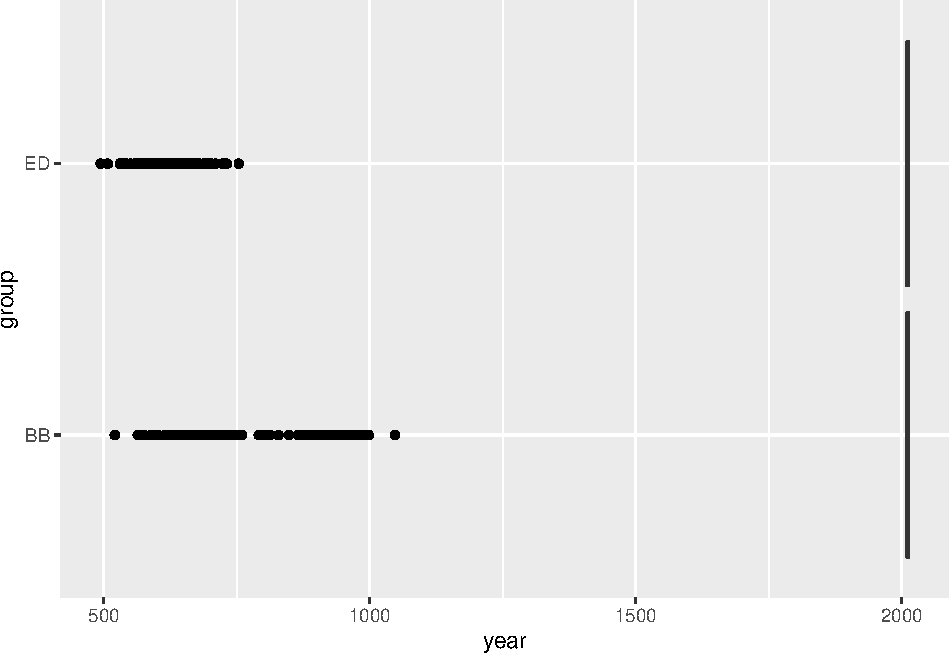
\includegraphics{analysis_files/figure-latex/e2-1-1.pdf}

\subsubsection{Exercise 2.2}\label{exercise-2.2}

\begin{itemize}
\tightlist
\item
  The data is from \href{https://doi.org/10.1017/S1360674323000047}{The
  decline of local anchoring: a quantitative investigation} and includes
  occurrences of prepositional phrases in different texts.
\item
  The English period labels are: ``OE'' = Old English, ``ME'' = Middle
  English, ``eModE'' = Early Modern English, ``lModE'' = Late Modern
  English. Make sure the order of the English periods reflects the
  historical order (as given here).
\end{itemize}

\begin{Shaded}
\begin{Highlighting}[]
\NormalTok{data\_e2\_2 }\OtherTok{\textless{}{-}} \FunctionTok{read\_csv}\NormalTok{(}\StringTok{"data/data\_e2\_2.csv"}\NormalTok{) }\SpecialCharTok{\%\textgreater{}\%}
  \FunctionTok{filter}\NormalTok{(}
\NormalTok{    Include }\SpecialCharTok{==} \DecValTok{1}
\NormalTok{  )}
\end{Highlighting}
\end{Shaded}

\begin{verbatim}
## New names:
## Rows: 21558 Columns: 34
## -- Column specification
## -------------------------------------------------------- Delimiter: "," chr
## (25): TextId, SubType, Title, Author, Genre, Cat, Locs, Locw, ft_clsMain... dbl
## (7): ResId, Date, Size, Words, ft_antdist, Include, TextList lgl (2): ...32,
## ...33
## i Use `spec()` to retrieve the full column specification for this data. i
## Specify the column types or set `show_col_types = FALSE` to quiet this message.
## * `` -> `...32`
## * `` -> `...33`
## * `` -> `...34`
\end{verbatim}

\begin{Shaded}
\begin{Highlighting}[]
\NormalTok{data\_e2\_2 }\SpecialCharTok{\%\textgreater{}\%}
  \FunctionTok{ggplot}\NormalTok{(}\FunctionTok{aes}\NormalTok{(EnglishPeriod, }\AttributeTok{fill =}\NormalTok{ Pentaset)) }\SpecialCharTok{+}
  \FunctionTok{geom\_density}\NormalTok{()}
\end{Highlighting}
\end{Shaded}

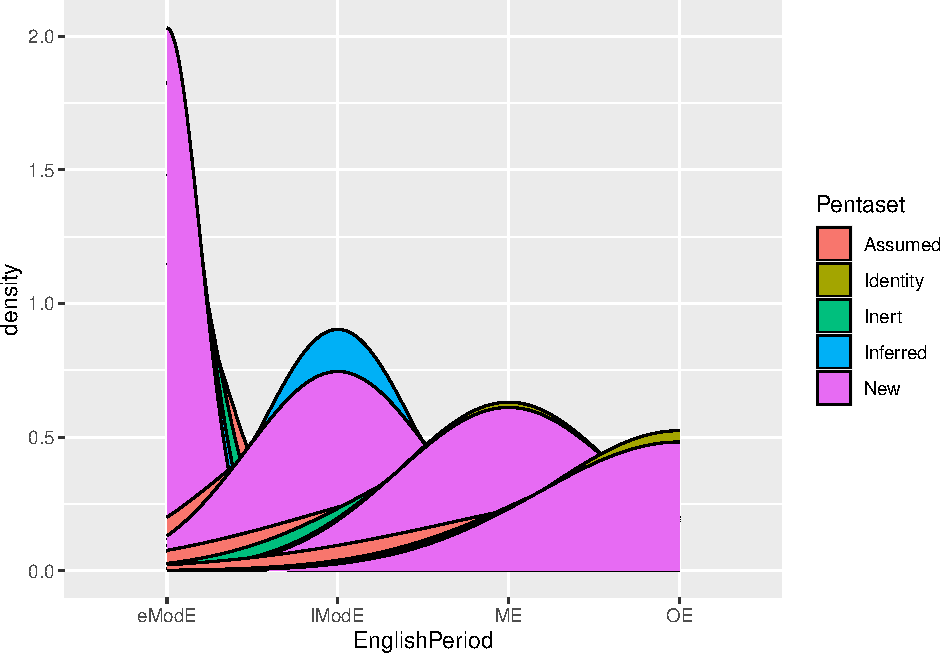
\includegraphics{analysis_files/figure-latex/e2-2-1.pdf}

\newpage

\subsection{Exercise 3: Choosing appropriate summary
measures}\label{exercise-3-choosing-appropriate-summary-measures}

\begin{itemize}
\tightlist
\item
  Read in \texttt{data\_e3.csv}. This is simulated data of P300
  measurements (Event Related Potential component P300) taken during an
  auditory odd-ball task by participants with Autistic Spectrum Disorder
  and a control group. The odd word in each trial differed by a set of
  features (controlled for as part of the experimental design), the
  number of which is recorded in \texttt{n\_feats} (from 1 to 4).
\item
  Obtain summary measures (central tendency: mean, median, or mode;
  dispersion: standard deviation or range):

  \begin{itemize}
  \tightlist
  \item
    For each variable on their own.
  \item
    For P300 in each group/response combination.
  \end{itemize}
\item
  Make sure to pick the correct measure(s) for the respective variable
  type.
\item
  Report all the measures in writing as you would in a paper.
\end{itemize}

\newpage

\subsection{Exercise 4: Identifying probability
distributions}\label{exercise-4-identifying-probability-distributions}

For each variable in the table below, specify in the ``Probability
distribution'' column whether it's (in principle) distributed according
to a Gaussian, a log-normal, or a Bernoulli distribution, or according
to some different one (put ``other'' in this case).

If you have doubts about any of the variables, you can write about it
briefly below the table.

\begin{longtable}[]{@{}
  >{\raggedright\arraybackslash}p{(\columnwidth - 4\tabcolsep) * \real{0.2361}}
  >{\raggedright\arraybackslash}p{(\columnwidth - 4\tabcolsep) * \real{0.5278}}
  >{\raggedright\arraybackslash}p{(\columnwidth - 4\tabcolsep) * \real{0.2361}}@{}}
\toprule\noalign{}
\begin{minipage}[b]{\linewidth}\raggedright
\end{minipage} & \begin{minipage}[b]{\linewidth}\raggedright
Variable
\end{minipage} & \begin{minipage}[b]{\linewidth}\raggedright
Probability distribution
\end{minipage} \\
\midrule\noalign{}
\endhead
\bottomrule\noalign{}
\endlastfoot
1 & Old vs young & \\
2 & Counts of verb occurrences & \\
3 & Hand (left vs right) & \\
4 & Entropy (0 to 1) & \\
5 & Reaction times (seconds) & \\
6 & Non-binary vs female vs male & \\
7 & Politeness (7 point scale from rudest to most polite) & \\
8 & VOT of voiceless stops & \\
9 & Logged word frequency & \\
10 & Number of f0 peaks & \\
\end{longtable}

\newpage

\subsection{Exercise 5: Critiquing and correcting a Bayesian linear
model}\label{exercise-5-critiquing-and-correcting-a-bayesian-linear-model}

Let's imagine a group of researchers decided to investigate whether
speech rate is affected by what kind of landscape you are viewing. You
are asked to review the paper where they describe their study and
results.

Here you can find the description of this mock study, including the
details of the Bayesian model the researchers have run. (The results are
not included.)

\begin{quote}
We recorded 50 subjects while they read 100 sentences on a screen. For
each subject, some of the sentences were presented together with videos
showing one of urban landscapes, natural landscapes, fireplaces, and
roller coasters.

For each trial we measured speech rate as number of syllables per second
(syl/s). The hypothesis is that speech rate will be faster in the roller
coaster setting relative to the urban setting, and slower in the natural
and fireplace settings relative to the urban setting. Moreover, we
expect that the natural and fireplace setting will have the same effect
on speech rate.

To assess these expectations, we ran a linear model using a Gaussian
distribution with setting as the outcome variable. We included speech
rate as the predictor. In R syntax:
\texttt{brm(setting\ \textasciitilde{}\ speech\_rate)}. We will use the
following treatment contrast coding:
\end{quote}

\begin{longtable}[]{@{}lllll@{}}
\toprule\noalign{}
& nature & fireplace & roller coaster & urban \\
\midrule\noalign{}
\endhead
\bottomrule\noalign{}
\endlastfoot
nature & 1 & 0 & 0 & 0 \\
fireplace & 0 & 1 & 0 & 0 \\
roller coaster & 0 & 0 & 1 & 0 \\
urban & 0 & 0 & 0 & 1 \\
\end{longtable}

Now critique the analysis (i.e., explain what is wrong with it in light
of the authors' hypotheses) and run a more appropriate linear model to
assess the research hypotheses of the study based on the provided data
(\texttt{data\_e5.csv}). Pay attention to the order of the levels in
\texttt{setting} (if you are unsure, carefully look at how the
hypotheses are formulated).

Feel free to also summarise and plot the data, although it is optional
and if you do you don't have to add it in the assessment (but you can if
you want to).

Report the model specification and the results of your linear model with
respect to the hypotheses (i.e.~do the results match the hypotheses or
not? Can we be certain?).

\end{document}
